\chapter{Resultater}
\begin{figure}[htbp]
    \centering
    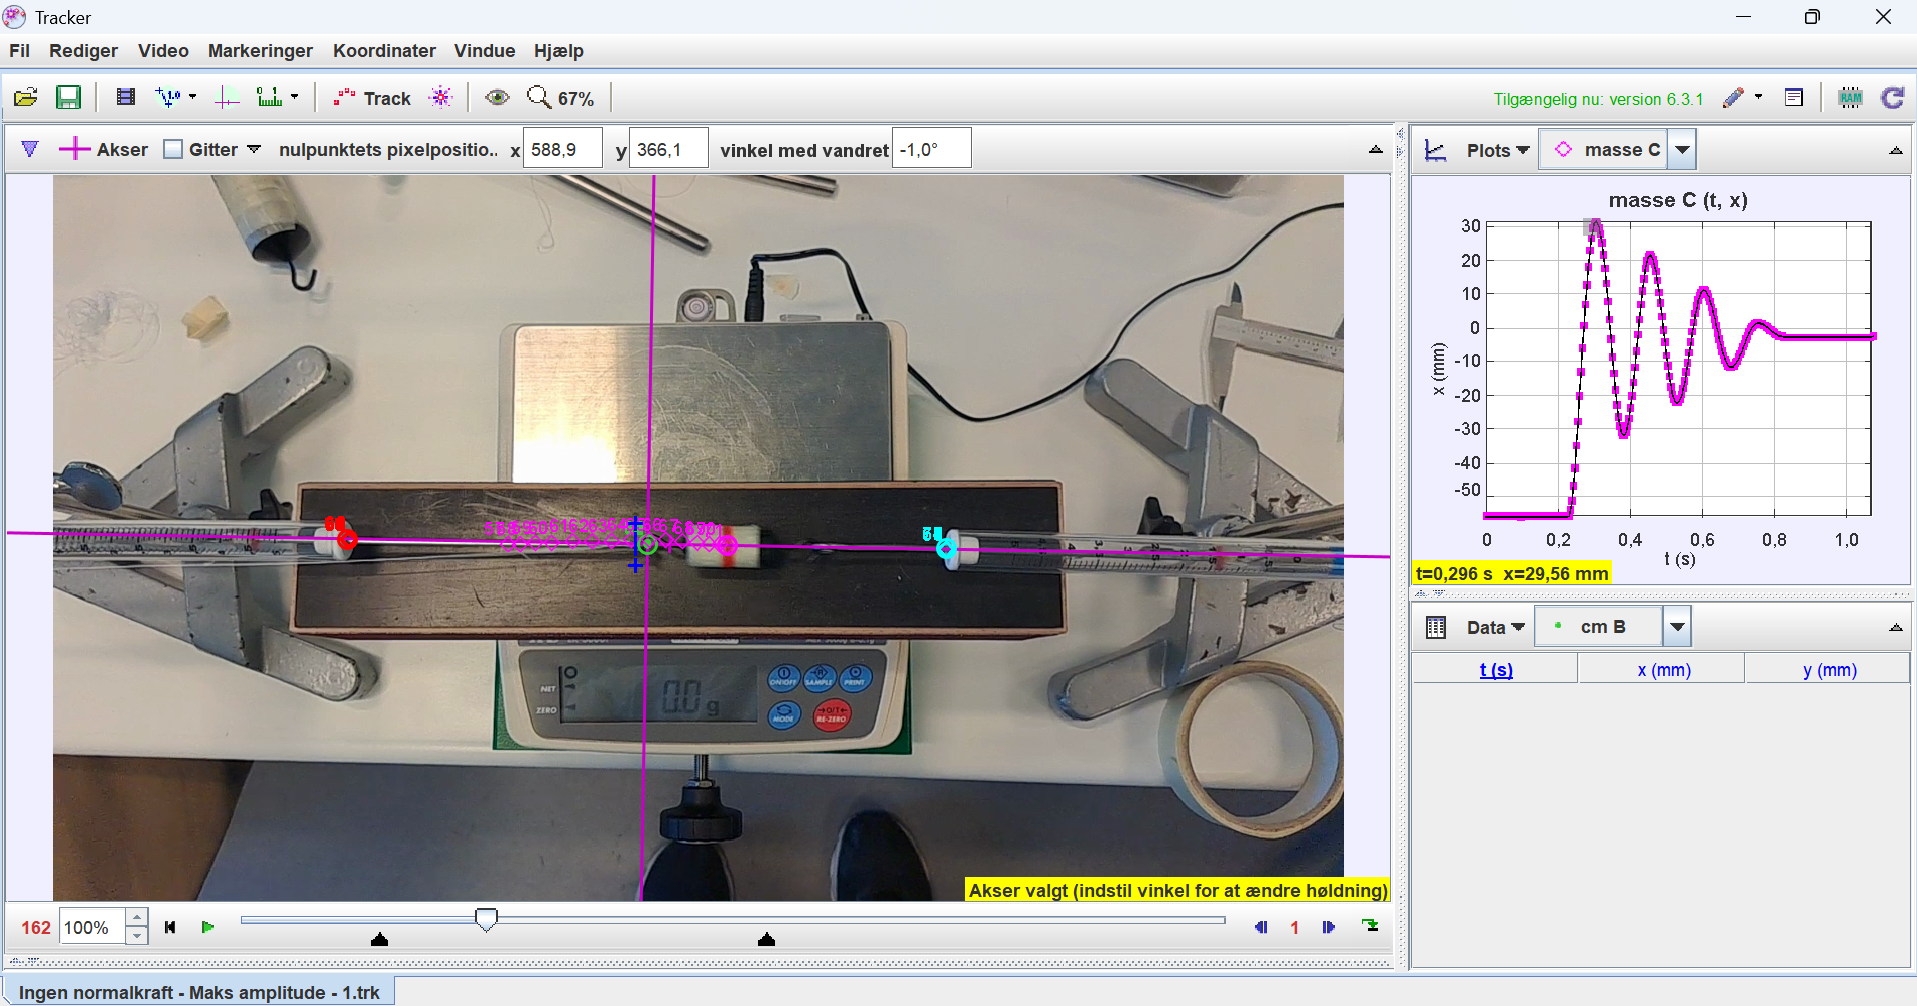
\includegraphics[width=0.8\linewidth,origin=c]{figures/data_eksempel.png}
    \caption{Eksempel på hvordan behandlingen af optagelserne ser ud i Tracker}
    \label{fig:tracker}
\end{figure}
Første skridt i behandlingen af optagelserne, var at køre dem igennem Tracker. 
Tracker er et program der kan bruges til at tracke objekter i en video, 
og vi brugte det derfor til at tracke bevægelsen af det røde bånd på loddet under svingningen.
Nulpunktet til trackningen, blev fundet ved at tracke de 2 ender af newtonmetrerne og så finde midtpunktet imellem dem, 
eftersom at de er lige stærke, så burde det være ligevægtspositionen (Vi vil senere se hvorfor dette er forkert).
Der medfølger mange usikkerheder med i brugen af Tracker. Den nok største er menneskelig fejl, 
idet man ved øjemål er nødt til at bestemme hvor midtpunktet af loddet er og hvor newtonmetrerne slutter,
og man skal selv indlægge en målestok i hver optagelse, hvilket vil sige at målestoksforholdene på hver måling nok afviger lidt fra hinanden. 
Afvigelserne er nok ikke meget større end nogle pixels, men den er helt sikkert tilstede.
\begin{figure}[htbp]
    \centering
    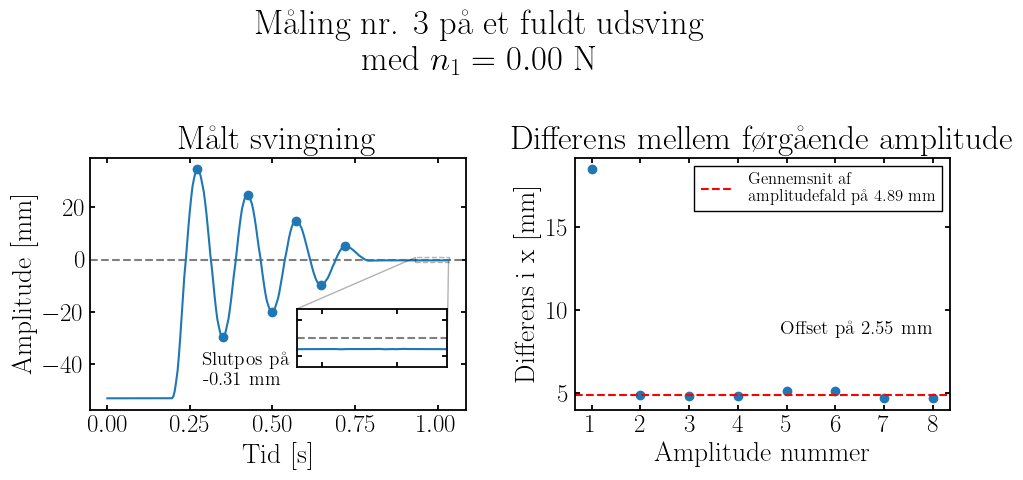
\includegraphics[width=0.8\linewidth,origin=c]{figures/n0.00-maks3.png}
    \caption{Databehandling uden offset}
    \label{fig:dårlig_graf}
\end{figure}
Bevægelsesdataen udvundet fra Tracker, har vi så brugt til at bestemme 2 ting. Vi har bestemt loddets slutposition, og alle dets toppunkter. 
Vi beregner så endvidere forskellen mellem 2 på hinanden følgende toppunkter, sådan at vi kan beregne hvor meget amplituden dæmpes (hypotesen var at det skulle være konstant).
Som der kan ses på figur \ref{fig:dårlig_graf}, ser selve bevægelsen ud som forventet, en svingning der gradvis dæmpes. 
Vi kan dog også se at dæmpningen per svingning er konstant (som forventet), men med en forskellig værdi i hver retning. 
Det ligner næsten af den er helt gnidningsfri i den ene retning, da amplituden ikke ændres, men endda stiger lidt i nogle af tilfældene.
Dette er meget i modstrid med hvad vi havde forventet, og også enormt urealistisk, at bevægelsen skulle være helt gnidningsfri i en af retningerne. 
Vi vil derfor tillade os at tilføje et kunstigt offset, da vi mistænker at nulpunktet er forkert placeret, får at undersøge hvilken effekt dette ville have. 
Dette gør vi ved at bestemme gennemsnittet af de høje værdier minus gennemsnittet af de lave, divideret med 4, da et offset får afstande fra top til bund til at falde med det dobbelte offset, 
og afstande fra bund til top ville stige med det dobbelte offset, altså tæller den med 4 gange. For eksempel, hvis de høje værdier lå på 10 og de lave på 0 (ligesom figur \ref{fig:dårlig_graf}),
ville vi bruge et offset på $\frac{10}{4}=2.5$, da de høje værdier dermed ville falde med 5, og de lave ville stige med 5, altså ville de begge ende ved den samme værdi som ønsket.
\begin{figure}[htbp]
    \centering
    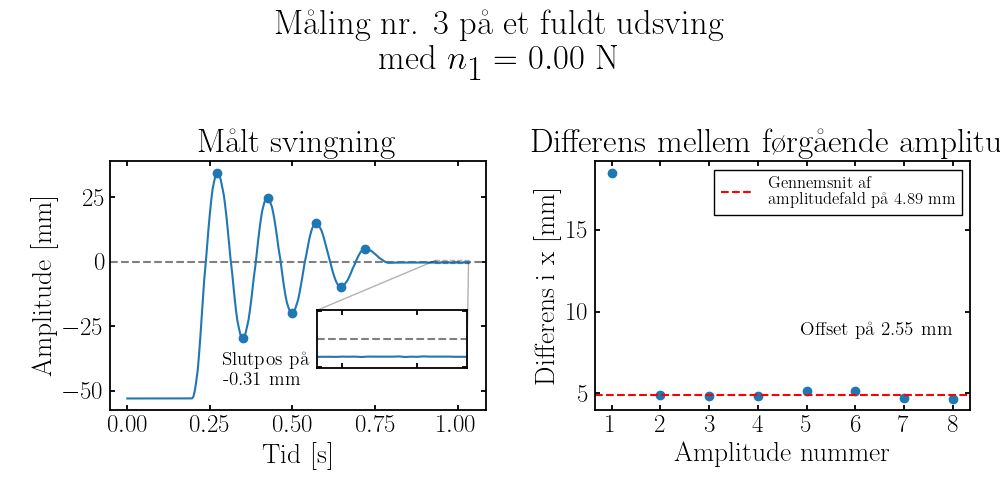
\includegraphics[width=0.8\linewidth,origin=c]{figures/n0.00-maks3-offset.png}
    \caption{Databehandling med offset}
    \label{fig:offset_graf}
\end{figure}
